\chapter{Phụ lục cơ sở dữ liệu}
\label{appendix:database_tables}

Phụ lục này tổng hợp các nội dung chi tiết liên quan đến cơ sở dữ liệu của hệ thống. Trong Chương~\ref{Chapter4}, báo cáo chỉ trình bày mô hình dữ liệu cốt lõi để giữ phần thiết kế gọn và dễ theo dõi. Phụ lục này bổ sung vị trí trình bày sơ đồ cơ sở dữ liệu đầy đủ và danh sách các bảng được đối chiếu từ các file schema và migration trong mã nguồn hiện thực của hệ thống.

\section{Sơ đồ cơ sở dữ liệu đầy đủ}

Sơ đồ cơ sở dữ liệu đầy đủ của hệ thống được đặt tại vị trí này để người đọc có thể đối chiếu với danh sách bảng chi tiết ở phần sau. Do sơ đồ đầy đủ có nhiều bảng và quan hệ, phần nội dung chính của báo cáo chỉ trình bày mô hình dữ liệu cốt lõi, còn sơ đồ đầy đủ được đưa vào phụ lục để phục vụ tra cứu.

% Khi có ảnh sơ đồ DB đầy đủ, có thể đặt vào đây, ví dụ:
% \begin{figure}[H]
% \centering
% \makebox[\textwidth][c]{%
%     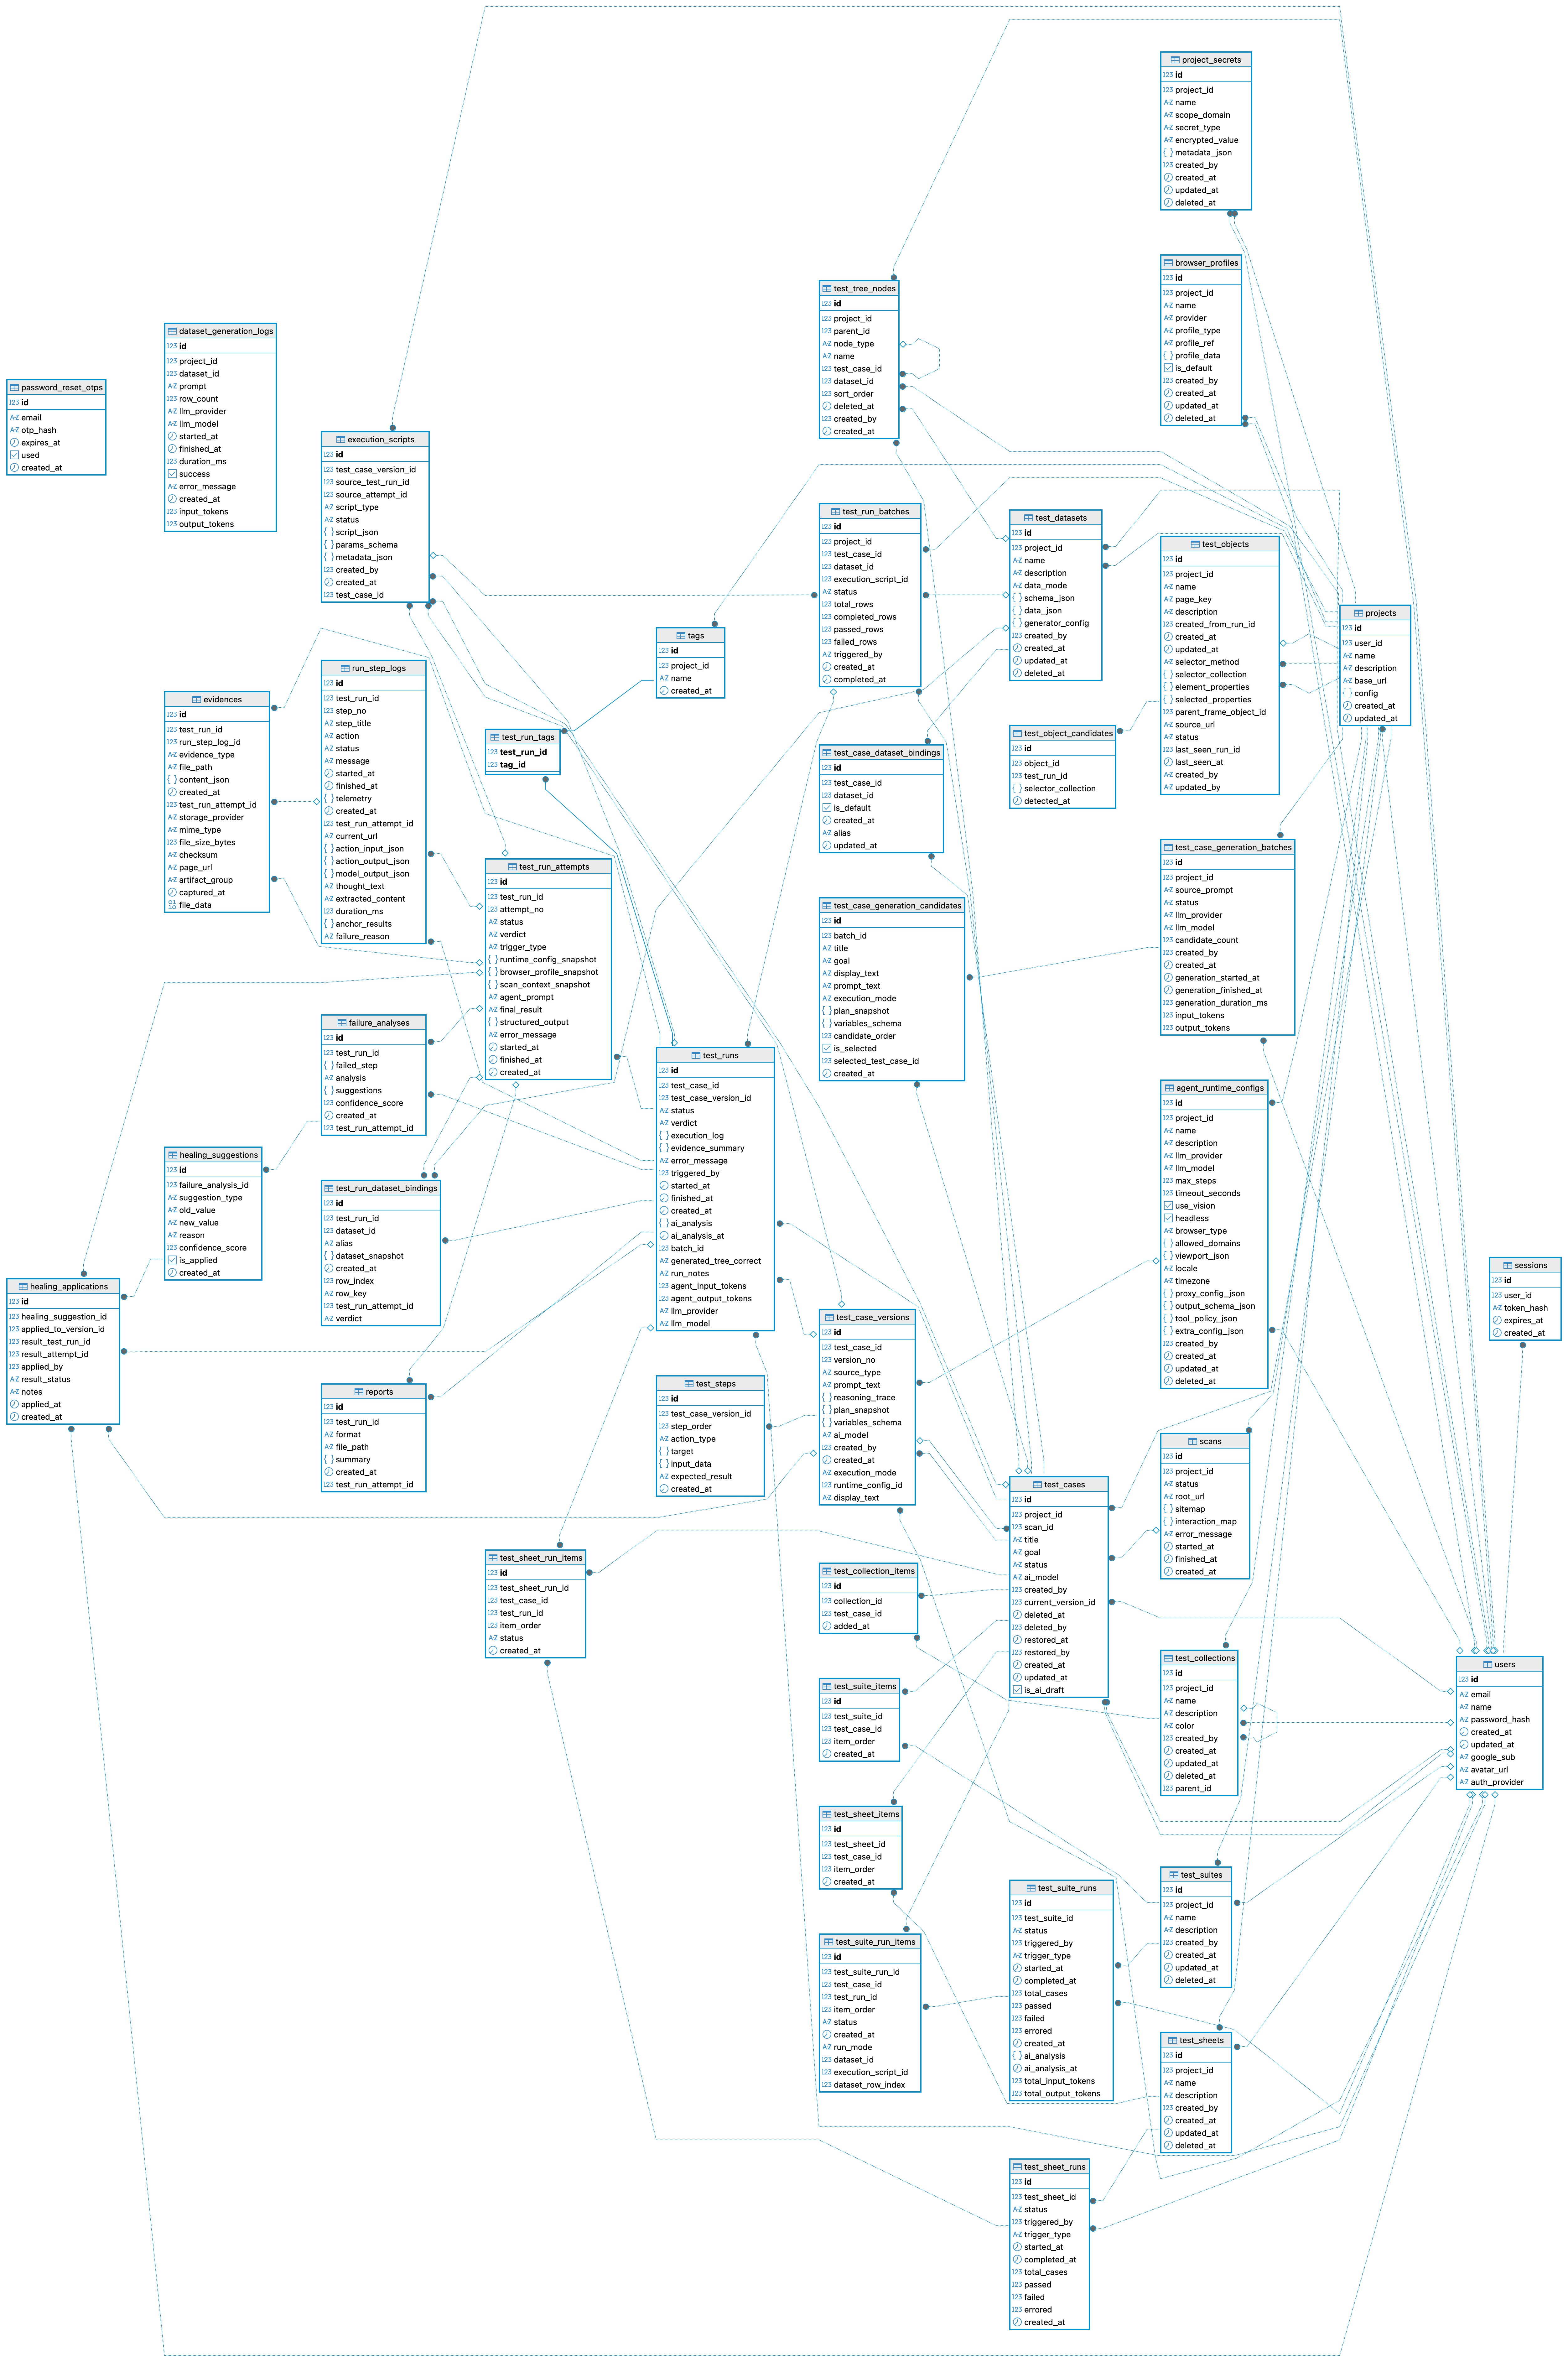
\includegraphics[width=1.15\textwidth]{images/appendix/db_full_diagram.png}
% }
% \caption{Sơ đồ cơ sở dữ liệu đầy đủ của hệ thống}
% \label{fig:appendix_db_full_diagram}
% \end{figure}

\section{Danh sách các bảng trong cơ sở dữ liệu}

{\scriptsize
\begin{longtable}{|p{3.2cm}|p{4.3cm}|p{6.7cm}|}
\caption{Danh sách các bảng trong cơ sở dữ liệu}
\label{tab:appendix_database_tables} \\
\hline
\textbf{Nhóm dữ liệu} & \textbf{Bảng} & \textbf{Vai trò chính} \\
\hline
\endfirsthead

\hline
\textbf{Nhóm dữ liệu} & \textbf{Bảng} & \textbf{Vai trò chính} \\
\hline
\endhead

Người dùng và bảo mật & \path{users} & Lưu tài khoản người dùng, thông tin đăng nhập, trạng thái onboarding và thông tin liên quan đến Google OAuth. \\
\hline
Người dùng và bảo mật & \path{sessions} & Lưu phiên làm việc hoặc thông tin hỗ trợ duy trì trạng thái đăng nhập. \\
\hline
Người dùng và bảo mật & \path{password_reset_otps} & Lưu mã OTP phục vụ chức năng quên mật khẩu và đặt lại mật khẩu. \\
\hline
Người dùng và bảo mật & \path{project_secrets} & Lưu dữ liệu nhạy cảm theo project như thông tin xác thực hoặc cấu hình bí mật cần kiểm soát truy cập. \\
\hline
Project & \path{projects} & Lưu project kiểm thử, base URL, mô tả, người sở hữu và cấu hình liên quan đến website mục tiêu. \\
\hline
Scan/crawl & \path{scans} & Lưu mỗi lần scan/crawl website, trạng thái, sitemap, interaction map, thời điểm chạy và lỗi nếu có. \\
\hline
Test case & \path{test_cases} & Lưu thông tin tổng quát của test case như tiêu đề, goal, project, trạng thái và phiên bản hiện tại. \\
\hline
Test case & \path{test_case_versions} & Lưu nội dung test case theo phiên bản, gồm prompt gốc, display text, plan snapshot, execution mode và cấu hình liên quan. \\
\hline
Test case & \path{test_steps} & Lưu các bước kiểm thử có cấu trúc gắn với test case hoặc phiên bản test case. \\
\hline
Test case & \path{test_tree_nodes} & Lưu cây test case hoặc cấu trúc phân cấp phục vụ biểu diễn và đánh giá nội dung sinh ra. \\
\hline
Sinh test case bằng AI & \path{test_case_generation_batches} & Lưu mỗi batch sinh test case từ prompt, gồm project, prompt, model, thời gian xử lý và thông tin token nếu có. \\
\hline
Sinh test case bằng AI & \path{test_case_generation_candidates} & Lưu các test case ứng viên được sinh ra trong một batch để người dùng xem, chỉnh sửa hoặc chọn lưu. \\
\hline
Sinh dataset bằng AI & \path{dataset_generation_logs} & Lưu log sinh dataset, prompt, trạng thái, số dòng dữ liệu, thời gian xử lý và thông tin token nếu có. \\
\hline
Replay script & \path{execution_scripts} & Lưu replay script được sinh từ phiên chạy agent thành công, gồm script JSON, metadata, tham số và trạng thái sử dụng. \\
\hline
Thực thi test & \path{test_runs} & Lưu mỗi lần chạy test case hoặc replay script, gồm trạng thái, verdict, thời gian chạy, lỗi tổng quát và người kích hoạt. \\
\hline
Thực thi test & \path{test_run_attempts} & Lưu từng attempt của một test run, gồm runtime snapshot, browser profile snapshot, trigger type và trạng thái attempt. \\
\hline
Thực thi test & \path{run_step_logs} & Lưu log từng bước thực thi như action, trạng thái, URL, error message, failure reason và thời điểm ghi nhận. \\
\hline
Thực thi test & \path{test_run_batches} & Lưu thông tin chạy theo lô hoặc batch replay, giúp gom nhiều test run thuộc cùng một yêu cầu thực thi. \\
\hline
Thực thi test & \path{test_run_tags} & Lưu quan hệ giữa test run và tag để hỗ trợ phân loại, lọc hoặc thống kê kết quả chạy. \\
\hline
Evidence và report & \path{evidences} & Lưu evidence như screenshot, DOM snapshot, console log, trace hoặc dữ liệu file/metadata artifact gắn với test run và step. \\
\hline
Evidence và report & \path{reports} & Lưu dữ liệu tổng hợp phục vụ màn hình báo cáo kết quả sau khi chạy test. \\
\hline
Evidence và report & \path{failure_analyses} & Lưu phân tích lỗi, failure type, ghi chú và gợi ý xử lý khi test thất bại. \\
\hline
Hỗ trợ phục hồi & \path{healing_suggestions} & Lưu gợi ý xử lý hoặc gợi ý sửa locator/script sau khi hệ thống phân tích lỗi. \\
\hline
Hỗ trợ phục hồi & \path{healing_applications} & Lưu việc áp dụng một healing suggestion và kết quả sau khi áp dụng. \\
\hline
Dataset & \path{test_datasets} & Lưu dataset ở dạng JSON tĩnh hoặc generator mode, gồm schema, dữ liệu và cấu hình sinh dữ liệu. \\
\hline
Dataset & \path{test_case_dataset_bindings} & Lưu quan hệ giữa test case và dataset được phép dùng hoặc dataset mặc định của test case. \\
\hline
Dataset & \path{test_run_dataset_bindings} & Lưu snapshot dataset được sử dụng tại thời điểm chạy test để truy vết dữ liệu đầu vào chính xác. \\
\hline
Test collection & \path{test_collections} & Lưu collection hoặc thư mục gom nhóm test case trong project. \\
\hline
Test collection & \path{test_collection_items} & Lưu các test case thuộc một collection và thứ tự hiển thị tương ứng. \\
\hline
Test sheet & \path{test_sheets} & Lưu nhóm test case theo dạng test sheet hoặc nhóm chạy cũ của hệ thống. \\
\hline
Test sheet & \path{test_sheet_items} & Lưu danh sách test case trong một test sheet và thứ tự chạy. \\
\hline
Test sheet & \path{test_sheet_runs} & Lưu mỗi lần chạy test sheet và kết quả tổng hợp của lần chạy đó. \\
\hline
Test sheet & \path{test_sheet_run_items} & Lưu kết quả từng test case con trong một lần chạy test sheet. \\
\hline
Test suite & \path{test_suites} & Lưu test suite phục vụ gom nhóm và chạy nhiều test case theo lô. \\
\hline
Test suite & \path{test_suite_items} & Lưu các test case thuộc một test suite và thứ tự chạy trong suite. \\
\hline
Test suite & \path{test_suite_runs} & Lưu mỗi lần chạy test suite, trạng thái tổng hợp và dữ liệu phân tích liên quan. \\
\hline
Test suite & \path{test_suite_run_items} & Lưu kết quả từng test case con trong một lần chạy test suite. \\
\hline
Object repository & \path{test_objects} & Lưu object giao diện theo project, gồm page key, selector collection, attribute snapshot và trạng thái xác nhận. \\
\hline
Object repository & \path{test_object_candidates} & Lưu các candidate locator hoặc candidate object được đề xuất cho một object hiện có. \\
\hline
Cấu hình chạy & \path{agent_runtime_configs} & Lưu cấu hình chạy agent như provider, model, timeout, số bước tối đa, viewport và allowed domains. \\
\hline
Cấu hình chạy & \path{browser_profiles} & Lưu cấu hình trình duyệt, profile type, profile reference và dữ liệu profile dùng khi chạy test. \\
\hline
Phân loại & \path{tags} & Lưu tag dùng để phân loại test run hoặc dữ liệu kiểm thử. \\
\hline
\end{longtable}
}

Danh sách trên tập trung vào các bảng nghiệp vụ và bảng hỗ trợ được ghi nhận trong schema/migration của hệ thống. Các bảng hệ thống của PostgreSQL, sequence và dữ liệu tạm sinh ra trong quá trình chạy không được liệt kê trong phụ lục này.
